% !TeX program = xelatex
\section{Java Spring Boot}
Das Backend in Spring-Boot bildet das Herzstück der ursprünglichen Software. Es stellt eine vollständige API für das Frontend bereit, bindet die PostgreSQL-Datenbank ein und kommuniziert mit den Kafka-Brokern. 
Ursprünglich handelte es sich um eine "CRUD-ähnliche" API, die neben den grundlegenden CRUD-Operationen auch das Starten und Stoppen von Projekten ermöglichte.

Da die Software jedoch noch auf Spring Boot 2.7.5 lief und daher den Übergang von JavaX zu Jakarta nicht vollzogen hatte, mussten zuerst alle Maven-Abhängigkeiten aktualisiert werden. Zudem war das Frontend noch Teil der Maven-Ziele. 
Da die Anwendungen jedoch separat voneinander ausgeführt werden müssen, musste dies ebenfalls entfernt werden.

Basierend auf der Anforderungsanalyse aus Kapitel \ref{cha:Anforderungsanalyse} werden hier drei der fünf vorgestellten Punkte behandelt. Da es sich um die erste API handelt, die lediglich erweitert wurde, waren viele der 
technischen Anforderungen bereits erfüllt. Die Einführung von Metriken für Prometheus und ein zentralisiertes Logging wurde mithilfe entsprechender Bibliotheken, Konfigurationsdateien und Annotationen schnell umgesetzt.

\subsection{Architekturentscheidung und Umstrukturierung}
Um die Architektur der Software flexibler zu gestalten, war eine Umstrukturierung in Richtung einer hexagonalen Architektur wichtig. Diese Architektur stellt eine Erweiterung der von Eric Evans in "Domain-Driven Design: 
Tackling Complexity in the Heart of Software" \cite{evans2004ddd} beschriebenen Domain-Driven-Architektur dar. Diese vierschichtige Architektur unterscheidet sich in einigen wesentlichen Aspekten von den zuvor genutzten Strukturen, 
in denen Pakete streng nach Entitäten strukturiert wurden und sowohl Datenbank-, Service- als auch Kommunikationsschichten integriert waren. Dies reflektierte das übliche Domain-Driven Design, bei dem Anwendungen in Präsentations-, 

Logik- und Datenschichten unterteilt werden, um "Concerns", also Aufgaben, getrennt voneinander zu behandeln. Beispielsweise darf nur die Logik-Schicht Änderungen an den Daten vornehmen, während die Datenbankschicht lediglich zum Schreiben und 
Lesen genutzt wird. In der ursprünglichen Architektur war dies jedoch nicht konsequent umgesetzt, und es gab viele Überschneidungen.

Um die Trennung der Zuständigkeiten konsequent umzusetzen, war eine Umstrukturierung erforderlich. Da bereits zu Beginn klar war, dass die Spring-API auch mit anderen Services kommunizieren muss, bot sich eine hexagonale Architektur an. 
Das Ziel der hexagonalen Architektur, auch bekannt als "Ports-und-Adapter-Pattern", besteht darin, die Trennung zwischen der Logikschicht und den externen Schichten zu verstärken und zu konkretisieren. Dies geschieht, indem Akteure über 
technologieagnostische Schnittstellen wie Interfaces kommunizieren. Diese "Ports" dienen daher als Schnittstellen zwischen den Schichten. Die Adapter sind die Initiatoren der Interaktionen, beispielsweise RestController, JPARepositories oder 
WebsocketController, die als Schnittstellen nach außen agieren.


%% caption \caption{Links ist die alte Datenstruktur, rechts die neue}
\begin{figure}[htbp]
    \centering
    \begin{minipage}{.48\textwidth}
        \adjustbox{valign=t}{
            \begin{forest}
                for tree={
                font=\ttfamily,
                grow'=0,
                child anchor=west,
                parent anchor=south,
                anchor=west,
                calign=first,
                edge path={
                        \noexpand\path [draw, \forestoption{edge}]
                        (!u.south west) +(7.5pt,0) |- node[fill,inner sep=1.25pt] {} (.child anchor)\forestoption{edge label};
                    },
                before typesetting nodes={
                        if n=1
                            {insert before={[,phantom]}}
                            {}
                    },
                fit=band,
                before computing xy={l=15pt},
                }
                [de.tudresden.sus
                    [project
                            [ProjectController.java]
                            [ProjectService.java]
                            [Project.java]
                    ]
                    [track
                            [TrackController.java]
                            [TrackService.java]
                            [Track.java]
                    ]
                    [dataSet
                            [DataSetController.java]
                    ]
                ]
            \end{forest}
        }
    \end{minipage}\hfill
    \begin{minipage}{.48\textwidth}
        \adjustbox{valign=t}{
            \begin{forest}
                for tree={
                font=\ttfamily,
                grow'=0,
                child anchor=west,
                parent anchor=south,
                anchor=west,
                calign=first,
                edge path={
                        \noexpand\path [draw, \forestoption{edge}]
                        (!u.south west) +(7.5pt,0) |- node[fill,inner sep=1.25pt] {} (.child anchor)\forestoption{edge label};
                    },
                before typesetting nodes={
                        if n=1
                            {insert before={[,phantom]}}
                            {}
                    },
                fit=band,
                before computing xy={l=15pt},
                }
                [de.tudresden.sus
                    [adapter
                            [inbound
                                    [rest]
                                    [error]
                                    [websocket]
                            ]
                            [outbound
                                    [repositories]
                                    [entities]
                                    [mapper]
                            ]
                    ]
                    [ports]
                    [service]
                ]
            \end{forest}
        }
    \end{minipage}
    \caption{Alte Datenstruktur (links) und neue (rechts)}
\end{figure}


Die Vorteile dieser Architektur sind vielfältig: Sie fördert die Entkopplung von Komponenten, vereinfacht Tests, ermöglicht eine flexiblere Entwicklung durch die ausschließliche Implementierung gegen Interfaces und 
zeigt eine hohe Anpassungsfähigkeit gegenüber Änderungen. Ein potenzieller Nachteil könnte in der erhöhten Komplexität liegen, die jedoch durch das Weglassen der Domain-Modelle stark reduziert wurde.

Die neu definierten Schichten haben klare und abgegrenzte Verantwortlichkeiten. Das Adapter-Layer fungiert als oberste Schicht und beinhaltet alle externen Funktionalitäten. Es wird in einen Inbound- und einen Outbound-Teil 
unterteilt: Der Inbound-Teil ist verantwortlich für alle eingehenden Anfragen wie REST-Requests oder WebSocket-Verbindungen. Der Outbound-Teil umfasst alle nach außen gerichteten Funktionen, z.B. die Datenbankkommunikation oder 
den RestClient. Die Unterscheidung zwischen Inbound- und Outbound-Adaptern wird vom Datenfluss innerhalb des Service Layers gesteuert. Adapter, die Daten in das Layer eingeben und somit steuern, gehören zu den Inbound-Objekten. Adapter, 
die nach außen gehen, also vom Service Layer angesprochen werden, gehören in den Outbound-Bereich.

Im Port-Layer erfolgt die Kommunikation zwischen den Schichten. Anstatt eines direkten Zugriffs der RestController auf die Service-Beans wird ein Interface bereitgestellt, wobei Spring die korrekte Bean injiziert. 

Dies mag zunächst überflüssig erscheinen, entspricht jedoch dem Prinzip der Dependency Inversion: Höherrangige Komponenten sollten nicht direkt auf niederrangigere zugreifen, sondern lediglich auf deren Abstraktionen. Dies ermöglicht die 
flexible Austauschbarkeit verschiedener Implementierungen des Interfaces und erleichtert das Testen. Auch können Komponenten einfach ausgetauscht werden, ohne Einfluss auf die darunterliegende Struktur zu nehmen. So kann beispielsweise die 
REST-Schnittstelle komplett durch Websockets ersetzt werden, wobei nur die jeweiligen Endpunkte implementiert werden müssen. Die Geschäftslogik bleibt davon unberührt. Ebenso kann die verwendete Datenbank problemlos ausgetauscht werden, da ihre Schnittstelle 
durch das jeweilige Datenbank-Interface abstrahiert wird.

Obwohl viele hexagonale Architekturen ein Domain-Layer enthalten, der Domain-Modelle mit erweiterter Funktionalität gegenüber den Datenbankmodellen enthält, wurde in diesem Projekt auf dieses Layer verzichtet. Dies wurde gemacht, da es eine unnötige 
Komplexität eingeführt hätte und aktuell nicht notwendig erscheint. Die erforderlichen Funktionalitäten werden bereits durch bestehende Mapper-Klassen abgedeckt.


\subsection*{Anpassung der Datenstrucktur}
%% TODO: Datenstruktur anpassen
Ein Umbau der Datenstruktur, wie sie bereits in \ref{cha:Anforderungsanalyse:Datenmanagement} angedeutet wurde, lässt sich in zwei wesentliche Teile aufteilen.
\subsubsection{Datensätze und Vererbung}
Ursprünglich verfügte die Anwendung über eine recht einfache und sehr lineare Datenstruktur, welche im folgenden ER-Diagramm in Abbildung \ref{fig:datamodel_old_version} gezeigt wird.

\begin{figure}[ht]
    \centering
    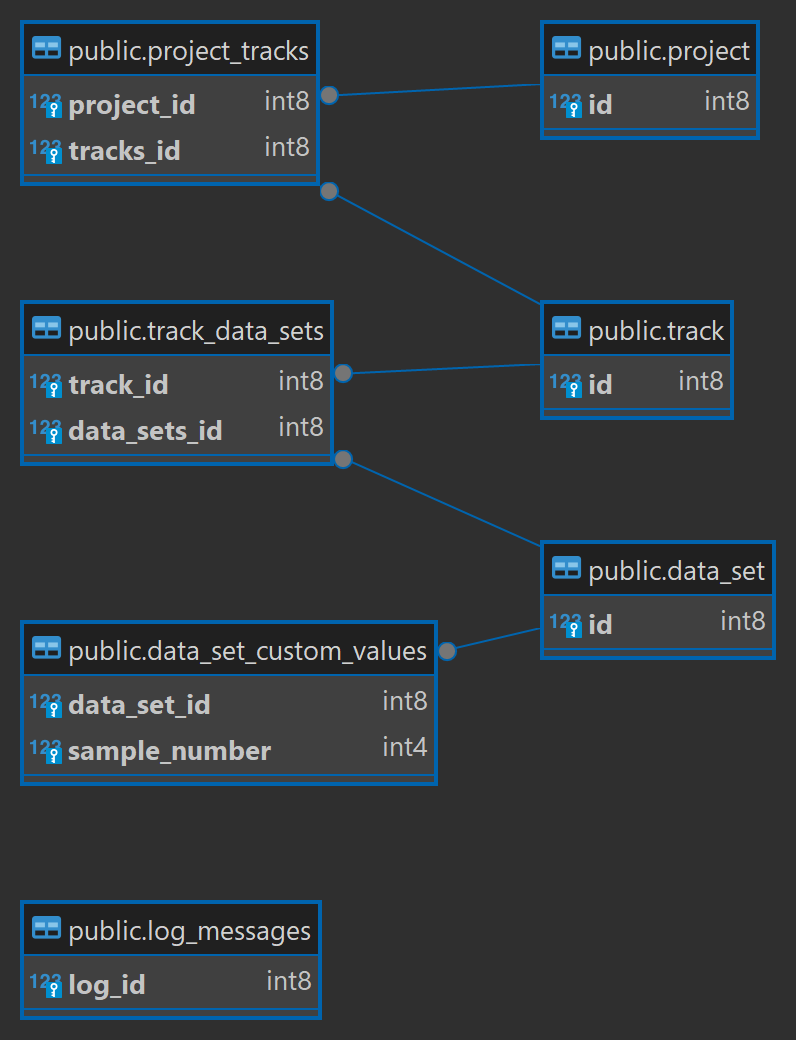
\includegraphics[width=1\textwidth]{includes/figures/database/software_old.png}
    \caption{Entity-Relationship-Diagramm der ursprünglichen Datenstruktur}
    \label{fig:datamodel_old_version}
\end{figure}



Diese Struktur bestand aus vier Komponenten: Ein Project ist in einer 1:n-Relation zu einem Track, der wiederum eine 1:n-Relation zu einem Datensatz hat. 
Diese Datenstruktur wurde ausgewählt, um komplexe Systeme modellieren zu können. Ein Project dient hierbei als Komponente, die mehrere datensendende Einheiten, 
sogenannte Tracks, umfasst. Da diese Tracks in unterschiedlichen Intervallen und insbesondere parallel senden können, war eine solche Unterscheidung notwendig. 
DataSets, aus denen ein Track besteht, fungieren als Abstraktionsebene der verschiedenen Phasen, in denen sich ein Track befinden könnte. So lassen sich durch aufeinanderfolgende DataSets unterschiedliche Situationen abbilden, 
beispielsweise die Simulation eines Gewächshauses (Project) mit drei Sensoren (Tracks) für Luftfeuchtigkeit, Temperatur und Lichtintensität. Die variierenden Bedingungen im Tagesverlauf, wie steigende und fallende 
Temperaturen, werden durch aufeinanderfolgende DataSets dargestellt. Jeder Track kann dabei eine eigene Frequenz besitzen.

Zur Nachverfolgung gesendeter Daten wird zudem ein Logverzeichnis angelegt.

Diese Herangehensweise erwies sich zwar als robust, jedoch auch als wenig flexibel. Die Art der zu sendenden Daten ließ sich nicht einfach anpassen, und die Zuweisung spezieller Eigenschaften zu unterschiedlichen 
Datentypen war nicht möglich. Die Beschränkung auf die in Trend, Residual und Season unterteilte Berechnungsvorschrift stellte eine weitere Limitierung dar.

Die erforderliche Flexibilität für die Erstellung komplexer Simulationsumgebungen und die Integration externer Konfigurationen, wie sie die Django-API ermöglicht, machte eine methodische Änderung notwendig. 

Hierfür wurden zwei Ansätze verfolgt:

\paragraph{Vererbung} 

Gemäß der in Listing \ref*{code:javaBaseDataSets} dargestellten Methode können neue Datensätze einfach von der Basisklasse erben. Neue Felder werden im selben Table gespeichert, wobei bei vielen neuen Feldern 
idealerweise eine neue Entität oder Entitätenstruktur erstellt werden sollte. Beim Auslesen aus der Datenbank wird dann über Casting die gewünschte Klasse rekonstruiert.
\begin{lstlisting}[language=Java, caption=Abstrakte Basisklasse der \textit{DataSets}, label={code:javaBaseDataSets}]
@Entity
@Inheritance(strategy = InheritanceType.SINGLE_TABLE)
@Accessors(chain = true)
@Data
@JsonTypeInfo(
        use = JsonTypeInfo.Id.NAME,
        include = JsonTypeInfo.As.PROPERTY,
        property = "type")
@JsonSubTypes({
        @JsonSubTypes.Type(value = CharDataSet.class, name = "char"),
        ...
})
@JsonAutoDetect(fieldVisibility = JsonAutoDetect.Visibility.ANY)
public abstract class PlainData implements DataTypeOption {

    @Id
    @Column(name = "id")
    @GeneratedValue(strategy = GenerationType.AUTO)
    private Long id;
    @Column(name = "position")
    private int position;
    @Column(name = "numSamples")
    private int numSamples;
    @Column(name = "frequency")
    private float frequency;
    @Column(name = "name")
    private String name;
    @Column(name = "dataType")
    private DataTypes dataType;
    ....
}
\end{lstlisting}


%% TODO neue DataSets einfügen und kurz erklären.


\paragraph{Polymorphe Deserialisierung} Um eine flexible Kommunikation zu gewährleisten, wird Jacksons polymorphe Deserialisierung eingesetzt\footnote{Jackson bietet eine umfangreiche Java API zum Arbeiten mit JSON}. Diese nutzt die in den 
\textit{@JsonSubTypes} definierten Optionen für das zielgerichtete Casting in die korrekten Objekte. Somit können die Objekte unabhängig vom Datentypen im Business-Layer verarbeitet werden und Typgerecht in der Datenbank gespeichert werden.

\begin{lstlisting}[language=Java, caption=Basisklasse der DTO Objekte, label={code:javaBaseDataSetsDTO}]
@JsonTypeInfo(
    use = JsonTypeInfo.Id.NAME,
    include = JsonTypeInfo.As.PROPERTY,
    property = "type")
@JsonSubTypes({
    @JsonSubTypes.Type(value = CharDataSetDTO.class, name = "char"),
    ...
})
@Data
@Accessors(chain = true)
@JsonAutoDetect(fieldVisibility = JsonAutoDetect.Visibility.ANY)
public class PlainDataDTO {

    @Schema(name = "id", nullable = true, minimum = "1")
    private Long id;
    ...
    
}
\end{lstlisting}


Jede Klasse muss außerdem eine eigene Mapper-Klasse bereitstellen, um die Datenstrukturen adäquat in die gewünschten DTOs zu konvertieren.

Die Implementierung dieser drei Klassen und ihrer Konfigurationen in den Basisklassen ermöglicht eine schnelle Erweiterung der bestehenden Datenstruktur. Zusätzlich implementieren alle Klassen ein Interface, das ihr jeweiliges Verhalten definiert. 
Dadurch kann eine neue Datenstruktur implementiert werden, ohne das Business-Layer zu beeinflussen. Wichtig ist, dass dieses Vorgehen den Grundsatz der Separation of Concerns nicht verletzt, da die neuen Datentypen lediglich eigene Datengenerierungsstrategien
implementieren, ohne das Verhalten außerhalb zu beeinflussen. Eine Ausnahme bilden die MLDataSet und TSADataSet, die ihre Daten extern (von der Django-API) beziehen. Hier wäre es theoretisch möglich, innerhalb der Entitäten einen REST-Client zu implementieren, 
was jedoch einen ungünstigen Datenfluss zur Folge hätte. Diese Aufgabe gehört eher zur Business-Logik und wird daher dort verarbeitet. Eine alternative Lösung wäre das Hinzufügen einer Domain-Schicht, die DataSets auf ein DomainModel projiziert. Da dies jedoch den 
Code unnötig aufblähen und bei den meisten DataSets diese Komplexität oder Abstraktion nicht benötigt wird, übernimmt das Business-Layer direkt diese Aufgabe.



\begin{lstlisting}[language=Java, caption={Mapper Klasse für DataSets, basierend auf den dataType, ein separates enum, fügen die Datentype eigenen mapper ihre Felder hinzu, bevor die global gültigen Felder gefüllt werden.}, label={code:javaBaseDataMapping}]
private final CharDataSetMapper stringMapper;
private final FloatDataSetMapper floatMapper;
private final IntegerDataSetMapper intMapper;
private final MlDataSetMapper mlMapper;
private final TSADataSetMapper tsaMapper;
private final CustomValueConverter customValueConverter;
private final SleepDataSetMapper sleepMapper;

public PlainData toEO(PlainDataDTO data) {
    var eo =  switch (data.getDataType()) {
        case FLOAT:
            yield floatMapper.toEO((FloatDataSetDTO) data);
        case CHAR:
            yield stringMapper.toEO((CharDataSetDTO) data);
        case INTEGER:
            yield intMapper.toEO((IntegerDataSetDTO) data);
        case ML:
            yield mlMapper.toEO((MlDataSetDTO) data);
        case TSA:
            yield tsaMapper.toEO((TSADataSetDTO) data);
        case SLEEP:
            yield sleepMapper.toEO((SleepDataSetDTO) data);
    };
    if (eo == null){
        throw new DataConversionException("cannot convert dto: %s".formatted(data));
    }
    return  eo.setId(data.getId())
                    .setFrequency(data.getFrequency())
                    .setName(data.getName())
                    .setNumSamples(data.getNumSamples())
                    .setPosition(data.getPosition());
}
\end{lstlisting}  


Über dieses System konnten problemlos der existierende Datentyp, welcher nur Fließkommazahlen unterstützte, durch neue Datentypen erweitert werden. Beispielsweise konnte die grundsätzliche Funktionalität dieses erhalten bleiben und durch eine Integer Konvertierung innerhalb der Logik zu einem IntegerDataSet erweitert werden.
Um Charactere zu versenden, musste die Funktion zur Generierung der Daten nur umgeschrieben werden, um die entsprechenden Zeichen aus dem gegebenen Alphabet zu generieren. Zum erstellen einer Pause sind weniger Daten relevant.
Hier sind weniger Daten relevant. Da dieses Element aber die Verhaltensweise des Codes verändert, sind hier auch Anpassungen im Business-Layer notwendig. Dieses muss nun die Pausen in den Stream einfügen.
Um die Ml-TSA bzw TSA-DataSets zu erstellen gilt grundsätzlich das gleiche Prinzip, nur sind hier weit mehr Daten relevant. Diese Komplexität wird auf die jeweiligen Mapper ausgelagert um die Separierung der Zuständigkeiten zu gewährleisten.

Eine Anforderung des Frontend sorgt nur für einen Bruch von Liskov Substitution Principle\footnote{Dieses Prinzip besagt, dass eine Superklasse }, da sich die neuen Datentypen nicht ganz wie das original Verhalten, bzw eine Implementation dieser Funktion schwer an die Anforderungen des Frontend anzupassen ist.
Wärhend im original das FloatingPointDataSet die Möglichkeit anbot, einen Vorschau der zu sendenden Daten zu erhalten und diese als Graph zu visualieren, ist dies über Chars oder Schlafzyklen schwer möglich. Hierfür müsste man die DataSets weiter über neue Interfaces aufspalten oder im Frontend eine neue Möglichkeit der Darstellung für solche Fälle finden.



\subsubsection{Eingabenvalidierung}
\label{sec:javaInputValidation}
Ein wichtiger Aspekt bei der Entwicklung einer API ist die Validierung der Nutzereingaben. Im ursprünglichen Projekt wurde sowohl auf Frontend-Validierung als auch auf Backend-Validierung Wert gelegt. 
Die Frontend-Validierung erfolgte über im React Code integrierte JSON-Schemata\footnote{JSON-Schemata sind ein IETF-Standard, der das Format und die Struktur eines JSON-Objekts definiert}, während im 
Backend Jackson verwendet wurde, um die JSON-Keys den entsprechenden Feldern zuzuordnen. Diese Methode funktionierte grundsätzlich, erwies sich jedoch als zu ungenau und unflexibel und bedurfte vor allem einer manuellen Validierung.

\paragraph{Anpassung der JSON-Schemata}
Um den neuen, komplexeren Anforderungen gerecht zu werden, war es notwendig, die JSON-Schemata aus dem Frontend zu entfernen und ins Backend bzw. in die Datenbank zu überführen. Die Schemata werden nun in der 
Datenbank gespeichert und von der API bereitgestellt. Dies bietet den Vorteil, dass Anpassungen an den Schemata vorgenommen werden können, ohne das Frontend neu bauen zu müssen. Zudem wird die Komplexität des Frontends reduziert, und Anpassungen an der Datenstruktur im Backend führen nicht mehr zu Komplikationen in der Kommunikation mit dem Frontend. Änderungen können direkt eingespielt werden, und durch entsprechendes Routing des Traefik kann die Datenstruktur überarbeitet werden, während eine alte Version noch läuft. Es muss lediglich nach dem Start des neuen Backend-Containers die Requests an ihn statt an den alten Container geleitet werden. Ein Nachteil ist die zusätzliche Serverbelastung, da die Schemata erst geladen und dann, abhängig von der Konfigurierbarkeit des DataSets, angepasst werden müssen, was zu Verzögerungen beim Nutzer führen kann. Angesichts der relativ geringen Datenmenge und den zielgerecht angepassten Schemata sowie passenderen Beschreibungen und Fehlermeldungen stellt dies jedoch einen akzeptablen Kompromiss dar. Darüber hinaus kann hier Caching zielgerichtet eingesetzt werden.

Ein wichtiger Schritt bei der Überführung der JSON-Schemata ins Backend war der Umstieg auf Hibernate ORM 6, das nun auch JSONB-Support für Postgres in Java bietet, ohne dass eigene Converter-Klassen erforderlich sind. 
Dies vereinfacht den Umgang mit JSON-Objekten im Java-Code erheblich.

\begin{lstlisting}[language=Java, caption=Neuer Umgang mit JSONB-Elementen in Java]
@Column(columnDefinition = "jsonb", name = "schema", nullable = true)
@JdbcTypeCode(SqlTypes.JSON)
private Map<String, Object> schema = new HashMap<>();
\end{lstlisting}

Über einen eigenen Service werden nun durch die Angabe des gewünschten DataTypes die JSON-Schemata dynamisch zusammengestellt. Dies beinhaltet das Hinzufügen und die Integration von Optionen, die zuvor über separate Anfragen gehandhabt wurden.

Beispielsweise haben nicht alle Machine-Learning-Modelle die Fähigkeit, Zukunftsprognosen zu erstellen. Da die Modelle jedoch alle derselben Kategorie angehören, wird für sie das gleiche Schema im Datenbankmodell gehängt. 
Hier muss das JSON-Schema dynamisch an die neuen Anforderungen angepasst werden. Normalerweise ist diese Option nicht vorhanden, daher muss der entsprechende Service sie nachträglich hinzufügen. Es gäbe auch die Möglichkeit, 
viele verschiedene Versionen der Schemata in der Datenbank zu speichern und zielgerichtet zu laden. Der Vorteil hier liegt in der Einfachheit und Versionierbarkeit. Darin liegt aber auch der Nachteil: Unterschiedliche Versionen 
müssen dennoch mit den zugrundeliegenden Datenstrukturen übereinstimmen. Eine dynamische Generierung über den Code hat dieses Problem nicht. Hier werden die Anforderungen der jeweiligen Version bereitgestellt. Es muss nur darauf 
geachtet werden, den Schema-Generator konsistent mit den Anforderungen des DataSets zu halten.

Ein weiterer Punkt, der grundlegend verändert wurde, ist der Umgang mit separaten Funktionen innerhalb der ursprünglichen DataSets. Im originalen Projekt gab es die Möglichkeit, diese durch die Optionen Residual, Season und 
Trend zu erweitern und zu konfigurieren. Dafür wurden mehrere Anfragen an das Backend gesendet, um die verfügbaren Optionen zu erhalten und anschließend je nach Auswahl der Option einen weiteren Request an das Backend gesendet, 
um das dafür vorgesehene Schema zu laden. Dies führte insgesamt zu einer geringeren übertragenen Datenmenge, die das Frontend verarbeiten musste, erhöhte jedoch den Aufwand für das Backend, da es mindestens sechs Anfragen bewältigen musste, 
um jeweils ein komplett konfiguriertes DataSet-Schema zu erstellen. Daher wurde auch dies geändert. Die jeweiligen Optionen sind nun Teil des initialen JSON-Schemas und werden durch die von JSON-Schema bereitgestellte Abhängigkeitsmethode dynamisch angezeigt.

\paragraph{Anpassung der Eingabenvalidierung im Backend}
\label{sec:java_bean_validation}
Die Eingabenvalidierung im Backend erfolgte ursprünglich allein durch Jackson und gelegentliche Null-Checks. Dies ist ausreichend, wenn ausschließlich über ein Frontend kommuniziert wird, das jegliche Validierung übernimmt. 
Für eine komplexere API ohne angemessene Eingabenvalidierung ist dieser Ansatz jedoch sehr unsicher und kann zu vielen, insbesondere für den Nutzer unklaren, Fehlern führen.

Jakarta bietet jedoch auch hierfür eine Lösung in Form der Bean-Validation, welche die JSR-380-Spezifikation\footnote{JSR 380 ist eine Java-API-Spezifikation zur Validierung von Beans, die Teil von Jakarta EE und JavaSE ist. 
Sie stellt sicher, dass Beans bestimmte Anforderungen erfüllen.} umsetzt. Über das spring-boot-starter-validation-Artefakt erhält man Zugriff auf Annotationen wie @NotNull, @Positive, @Size und weitere, die eine direkte Validierung der DTOs ermöglichen. 
Zudem werden Fehlermeldungen an die jeweiligen Exceptions weitergeleitet. Somit greift die in Sektion \ref{sec:java_error_handling} beschriebene Fehlerbehandlungsstrategie, und der Nutzer erhält direktes Feedback zu seinen Eingabefehlern.


\subsection{Fehlerbehandlung}
\label{sec:java_error_handling}
Ein wichtiger Aspekt ist der Umgang mit Fehlern. Fehler müssen, sofern möglich, dem Nutzer klar und strukturiert Mitgeteilt werden.
In einer REST API heißt dies, dass im Fehlerfalle dem Nutzer eine ErrorMessage übergeben wird, warum die Eingabe oder Anfrage nicht aktzeptiert oder bearbeitet werden kann.

Dafür mussten im ursprünglichen Projekt auch viele Änderungen vorgenommen werden. Einserseits wurde wie in Paragraph \ref{sec:java_bean_validation} beschriebene eine Bean Validation eingefügt.
Diese Kontrolliert bereits beim Eingang der Objekte, ob alle Krieterien erfüllt sind, wie beispielsweise das richtige Format, ob Zahlen positiv sind oder ob Namen einem gewissen Regex Muster folgen.
Sollte dies nicht der Fall sein, wird eine Exception geworfen, welche von einem eigenen ExceptionHandler abgefangen wird.

ExceptionHandler sind ein zentrales Element in der Fehlerverarbeitung.
Sie helfen enorm bei der Umsetzung des Fail Fast Prinzips\cite{fail_fast:online}, welches prinzipiell besagt, dass Fehler möglichst schnell behandelt und die bearbeitung abgebrochen werden soll.

Um die geworfenen Exceptions in verständliche ErrorMessage zu konvertieren und dem Nutzer zu senden bietet Spring die besagten ExceptionHandler. Diese fangen die geworfenen Exceptions ab und erstellen daraus passende Antworten.


\begin{lstlisting}[language=Java, caption={Error Handling für den Fall, dass Ids nicht gefunden werden}, label={code:javaErrorHandling}]
    @ControllerAdvice
    @Slf4j
    public class EntityNotFoundExceptionHandler {
        @ExceptionHandler(EntityNotFoundException.class)
        public ResponseEntity<RestError> handleEntityNotFoundException(
            final EntityNotFoundException ex) {
            log.error("Entity not found: {}", ex.getMessage());
            return new ResponseEntity<>(new RestError()
                    .setMessage(ex.getMessage())
                    .setError("INVALID_ID") 
                    .setI18nKey("INVALID_ID"),
                HttpStatus.NOT_FOUND);
        }
    }
\end{lstlisting}

In Listing \ref{code:javaErrorHandling} ist ein Beispiel für einen solchen ExceptionHandler zu sehen. Dieser fängt die EntityNotFoundException ab, welche geworfen wird, wenn eine Id nicht gefunden werden kann.
Um diesen Fehler zu internationalisiern, wird ein i18nKey mitgegeben, welcher in der entsprechenden Sprachdatei nachgeschlagen wird und dem Nutzer die entsprechende Fehlermeldung in seiner Sprache anzeigt.



\subsection{Absicherung der Anwendung über Spring Security}
%% TODO refresh-token erklären
\paragraph{Nutzerverwaltung und Anmeldung}
Ein entscheidender Aspekt bei der Entwicklung einer Webanwendung ist die Nutzerverwaltung und die damit verbundenen Sicherheitsanforderungen. Das ursprüngliche Projekt, obwohl als Webanwendung konzipiert, hatte keine Nutzerverwaltung implementiert. 
Dies führte dazu, dass jeder Nutzer Zugriff auf alle Projects, auch die von anderen Nutzern erstellten, hatte, ohne eine valide Möglichkeit, anderen Nutzern den Zugriff auf eigene Projekte zu verwehren.
Es Bot die Möglichkeit Projects hoch- und runter zu laden, eine etwas aufwändige Möglichkeit den Zugriff einzuschränken.

Die Integration eines \textit{User}-Elements in das Datenbankmodell war daher unumgänglich. User-Objekte nehmen nun die zentrale Rolle ein, da Projects, und somit auch die darunter liegenden Entitäten, an das Objekt gebunden sind. 
Um sicherzustellen, dass jeder Nutzer nur Zugriff auf seine eigenen Projekte hat, müssen daher Nutzerdaten an den Requests hängen. Es bietet sich daher an, ein grundsätzliches Nutzerauthentifizierungkonzept zu implementieren.
Hierfür wird Spring Security eingesetzt, ein Framework für Authentifizierung und Autorisierung, das auch Schutz vor gängigen Angriffen bietet. Es wurde konfiguriert, um JSON Web Tokens (JWT) zu erstellen und zu validieren, 
die nach erfolgreicher Anmeldung mittels E-Mail und Passwort dem Nutzer bereitgestellt werden.

Die Nutzung von JWT bietet mehrere Vorteile: Sie sind stateless, was bedeutet, dass der Server keine Session-Informationen speichern muss. Da JWT signiert sind, können sie als valide angesehen werden, solange das Secret sicher ist. Zudem sind sie unabhängig von der 
Anwendung einsetzbar, was besonders für das Zusammenspiel mit der Django API wichtig ist.
JWTs bieten jedoch auch Nachteile: Sie sind nicht widerrufbar, was bedeutet, dass ein einmal gestohlener JWT weiterhin gültig ist und von dritten Nachgenutzt werden kann. 
Zur minderung des Risikos besitzen sie daher nur eine kurze Lebensdauer (time to live, TTL).
Refresh-Tokens können hierbei helfen, da sie eine längere Lebensdauer besitzen und somit die Anzahl der notwendigen Anmeldungen reduzieren. Diese werden nur gesendet, sofern der JWT-Token abgelaufen ist.

Im Vergleich zu anderen Authentifizierungsmethoden wie LDAP ist die Integration von JWT einfacher und weniger aufwändig in der Konfiguration. Da JWT eine begrenzte Lebensdauer (time to live, TTL) haben, sind sie sicherer als API-Schlüssel, 
die regelmäßig erneuert werden müssen. Diese Notwendigkeit zur regelmäßigen Erneuerung war ein wichtiger Faktor bei der Entscheidung, JWT auch für die Django-API zu implementieren und zu konfigurieren.

Eine weitere Option wäre OAuth2.0 gewesen, ein weit verbreitetes Autorisierungsframework, das den Zugriff für Drittanbieteranwendungen ermöglicht. Trotz seiner Verbreitung wurde es aufgrund der hinzugefügten Komplexität nicht für die Integration in das Projekt ausgewählt.

\paragraph{Konfiguration von Spring Security}
\label{sec:javaSpringSecurityConfig}
Cross-Origin Resource Sharing (CORS) und Cross-Site Request Forgery (CSRF) stellten viele Herausforderungen während des Entwicklungsprozesses dar. Nachdem das ursprüngliche Projekt aufgespalten und Axios im Frontend integriert wurde 
(siehe \ref{sec:frontendCommunication}), traten erstmals CORS-Probleme auf, da das Frontend und das Backend nun über unterschiedliche IP-Adressen im Docker-Netzwerk kommunizierten.

Anfangs wurde das Problem durch die Verwendung der Annotation @CrossOrigin behoben, was jedoch nur eine temporäre Lösung war. Spätere Probleme bei der Konfiguration mit NginX wurden schließlich durch Spring Security gelöst. Mit der Implementierung von 
Spring Security 6 kam auch die überarbeitete Version der SecurityFilterChain, die das Injizieren von frei konfigurierbaren CorsConfigurationSource Beans ermöglicht. Ihre erlaubten Origins können über die application.properties und damit über Umgebungsvariablen gesteuert werden.

Die Security-Chain kümmert sich auch um die Nutzervalidierung. Hierfür muss lediglich der eigene AuthenticationProvider als Bean injiziert werden. Dieser implementiert den OncePerRequestFilter und prüft den anhängenden JWT auf sein Ablaufdatum und validiert ihn.
Refresh-Tokens werden über einen eigenen Endpunkt validiert und erneuert.

\paragraph{Anbindung des Nutzers an die Datenstruktur}
Die Anbindung des Nutzermodells an die bestehende Datenstruktur erfolgte, ohne den bestehenden Code groß anzupassen, aus zwei Gründen: Einerseits erleichtert es die Entwicklung, wenn der Fokus nicht auf Sicherheit liegt, andererseits ist es auch nicht die 
Aufgabe des Business Layers, sich um die Sicherheitsaspekte zu kümmern. Da die Nutzervalidierung über JWT bereits im Paragraph \ref{javaSpringSecurityConfig} stattgefunden hat, bevor die Requests an den jeweiligen RestController gehen, filtert Spring Security die Anfragen vorab.

Um den Nutzer dennoch an die Projekte zu binden, wurde ein aspektorientierter Programmieransatz gewählt. Dieser Ansatz, ein Paradigma innerhalb der objektorientierten Programmierung, versucht, Funktionalitäten über mehrere Klassen hinweg zu verwenden. Dies geschieht über eine Annotation, die an die gewünschte Methode angehängt werden muss. Da die Kommunikation mit der Datenbank über JpaRepository-Interfaces stattfindet, kann das Filtern nach Nutzern über das Ausnutzen von Default-Methoden in den Interfaces implementiert werden, ohne den restlichen Code anzutasten.

Die in Listing \ref*{code:javaSecurityDataBaseAccess} dargestellte Annotation @AttachUser zeigt einen Spring-Interceptor, der Spring signalisiert, dass hier eine Aktion eingewoben werden muss. In der Terminologie der aspektorientierten Programmierung handelt es sich bei der Methode findById(), sowie jeder anderen Methode, um einen Joinpoint. Durch den Pointcut, welchen die @AttachUser-Annotation liefert, wird ein Aspekt (der UserAspect) auf eine Advice gemapped, die von der Annotation selbst bereitgestellt wird.

Da Tracks und deren DataSets an das jeweilige Projekt gebunden sind, ein Zugriff ohne JWT nicht möglich ist und das User-Objekt an die Datenbankabfragen gebunden wird, ist somit ein Zugriff auf fremde Projekte ausgeschlossen.


\begin{lstlisting}[language=Java, caption={Annotation um einen Advice Annotation zu signalisieren}, label={code:javaSecurityDataBaseAccess}]
@Retention(RetentionPolicy.RUNTIME)
@Target(ElementType.METHOD)
public @interface AttachUser {
}
\end{lstlisting}


\subsection{Bidirektionale Kommunikation mittels Websockets}
\label{sec:javaWebsocket}

Nutzer mögen es visuelles Feedback zu bekommen, gerade bei Aktionen, deren direkten Verlauf sie nicht sehen können. 
Dieser Fall tritt ein, wenn der Nutzer die Daten an Kafka sendet, da dies über einen längeren Zeitraum stattfindet und, abhängig von den Konfigurationen, veränderlich ist.
In der alten Version wurde das Senden von Inhalten über eine Status LED angedeutet, welche blinkte, sobald Daten gesendet wurden. Dies ist aber nur eine sehr grobe Anzeige, welche dem Nutzer nur bedingt weiterhilft.
Da sie über einen Status in der ProjektResource angesteuert wurde, konnte sie auch nicht anzeigen ob der Sendevorgang bereits abgeschlossen ist.

Um solche Funktionalitäten zu ermöglichen bedarf es einer bidirektionale Kommunikationsschicht. 
Im Gegensatz zu REST, welches auf dem Request-Response Prinzip basiert, ist Websocket eine bidirektionale Kommunikationsschicht, welche auf dem Publish-Subscribe Prinzip basiert und somit die Kommunikation 
in beide Richtungen ermöglicht. Somit kann der Server den Client über den aktuellen Status in real time informieren.


Der Einsatz von Websockets hat zu ein paar Problemen geführt, Websockets unterschützen keine AuthorizationHeader, weshalb der in Sektion \ref{sec:javaSpringSecurityConfig} erläuterte 
Validierungsprozess nicht mit Websockets funktionierte, da normale Websocket keinerlei Header benutzen.
Somit musste der Loginprozess, für die Websocket Controller, neu definiert werden.
Um die Validierung ähnlich früh abzufangen wie im JWT Prozess musste daher ein einener WebsockerJWTHandler implementiert werden, welcher den initialen ServerHttpRequest nimmt und über auf einen token QueryParameter prüft. Für diesen QueryParameter wird der JWT genutzt.
Es wird nur beim ersten connection Aufbau geschaut ob der JWT gültig ist, websockets führen keine weitere Authentifizierung weiter durch. 
Dies ist aber im Bezug zur Aufgabe, welche die Websockets übernehmen müssen, auch sehr passend. Die langen Tasks sollten nicht durch ablaufende Authorisierungskeys behindert werden.

Ist eine Websocket Connection erstellt, wird das senden vorbereitet. Dies bedeutet, dass alle DataSets aus ihrern Konfigurationen Daten erstellen und diese in einem speziellen Objekt ablegen.
Sollte es sich bei den DataSets um MLDataSets oder TSADataSets handeln, muss hierfür ein RESTCall zur Django API getätigt werden (siehe Sektion \ref{sec:javaRestClient}).

Da die Elemente auf verschiedenen Threads arbeiten, müssen die aktuellen Statusinformationen Event gesteuert versendet werden. 
Dies bedeutet aber auch, das diese Stelle auch einen direkten Überblick darüber hat, welcher Thread gerade welches DataSet versendet.


\begin{figure}[h]
    \centering
    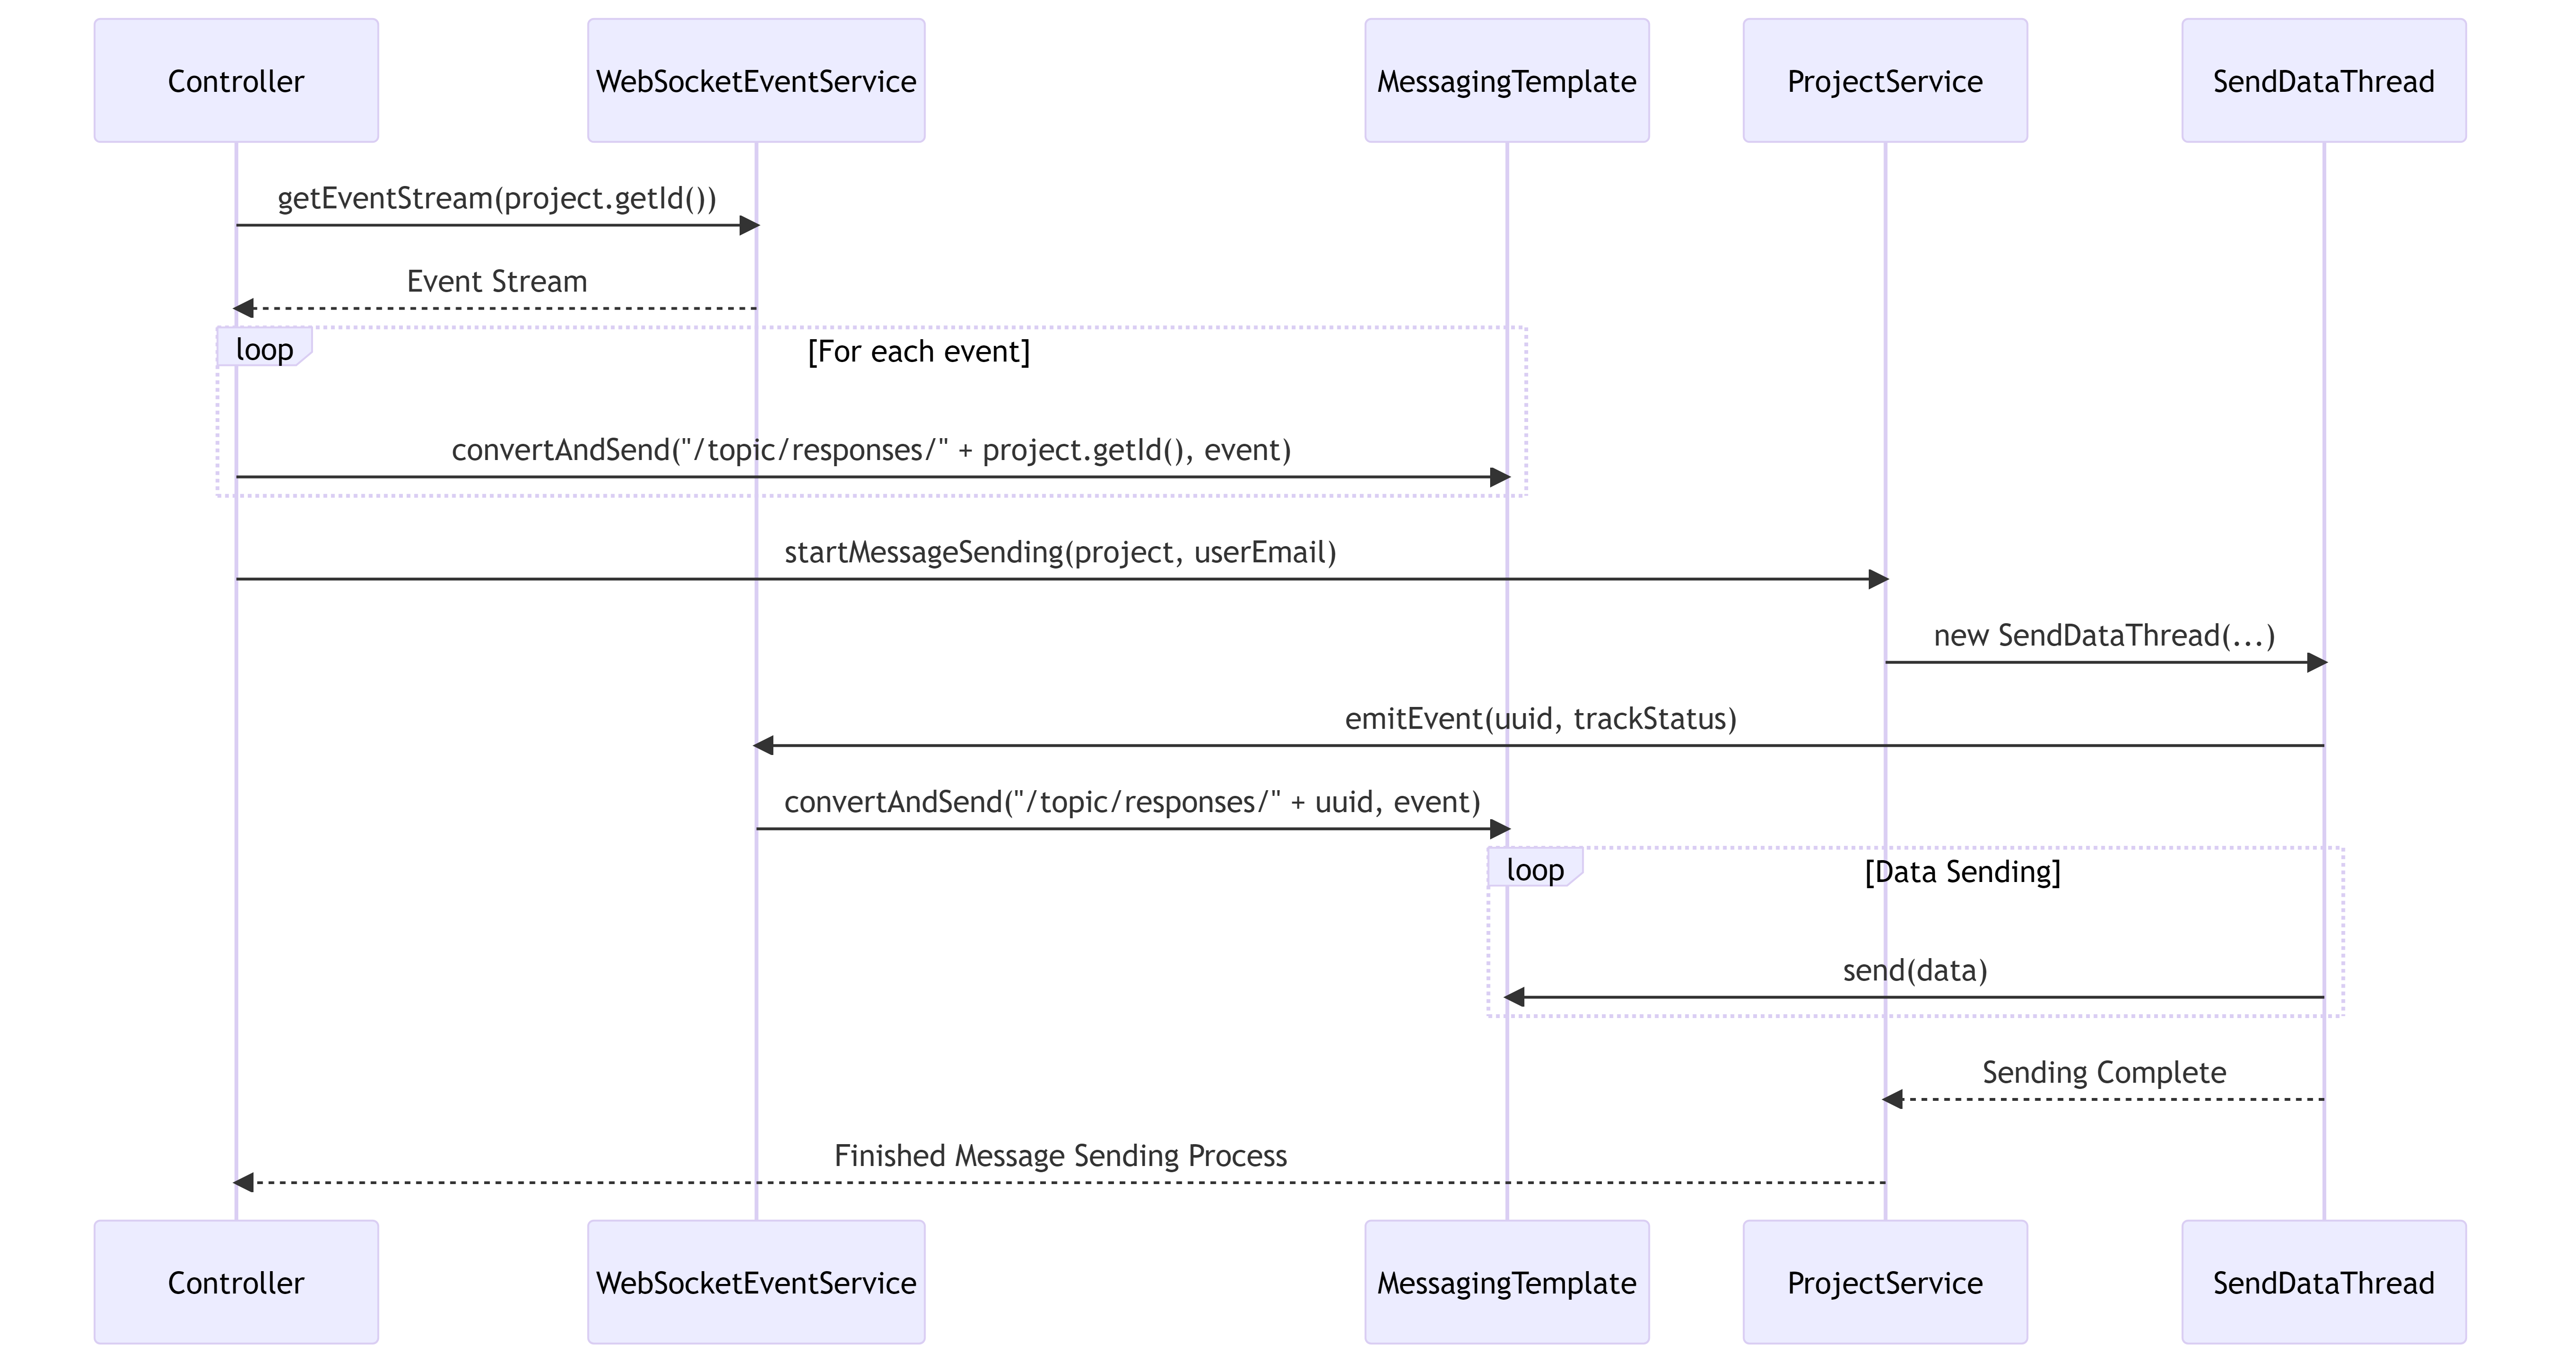
\includegraphics[width=1\linewidth]{includes/figures/EventService.png}
    \caption{vereinfachter Ablauf des Sendens von Statusinformationen mittels eines eigenen EventServices}
\label{fig:java_event_service}
\end{figure}

Hierzu wurde ein eigener EventService eingerichtet, welcher über den aktuellen Fortschritt von allen Threads informatiert wird.
Wie in Figur \ref{fig:java_event_service} zu sehen ist, informieren die einzelnen Threads den EventService über einen wechsel des sendenden DataSets innerhalb eines Tracks.





\subsection{Kommunikation mit der Django API über REST-Clients}
\label{sec:javaRestClient}
Microservices zeichnen sich dadurch aus, dass sie unabhängig voneinander agieren und arbeiten können. Die Kommunikation ziwschen den Services erfolgt über RESTCalls.
Da in der aktuellen Architecktur nur der Spring Service Daten vom Django Service nutzt, muss in Spring hierzu einen RESTClient implementieren, welcher die Anfragen an den anderen Service sendet und die Antworten verarbeitet.

Die Kommunikation zwischen den Services wird über JSON geregelt, wodurch die Kommunikation unabhängig von der Programmiersprache ist.

Anfänglich wurde hierfür die Webflux API von Spring verwendet, da die reine WebClient API nicht ausreichend war und den Implementationsaufwand unnötig erhöht hätte.
Mit der Version 3.2.0 von Spring boot wurde eine neue WebClient API eingeführt, welche Funktional ähnlich der in Quarkus genutzten RestClient API\footnote{https://quarkus.io/guides/rest-client-reactive} ist und daher die Nutzung erleichtert (durch Reduktion des Boilderplate Codes) und das automatische Entitätsmapping übernimmt, wurde die Webflux API durch die neue WebClient API ersetzt.

Der WebClient kommt auch mit einer Failsafe API, auf die aber verzichtet wurde.
Fehlercodes werden durchgereicht, aber erneutes senden von Requests wird nicht durchgeführt. Sollte die DjangoAPI nicht erreichbar sein, wird nur der Fehler an den Nutzer weitergegeben. 
Erneutes senden von Requests würde, sofern die Django API noch existiert, diese nur weiter belasten und der Nutzer wäre von enormen Delays betroffen, welche seine Konfiguration unvorhersehbar machen würden. Dies ist Kontraproduktiv.
Unvollständige DataSets zu senden ist auch keine valide Strategie, da dies im zu testenden System zu ungewollten Verhalten führen würde.
